\section{Transformer \& Conformer in ASR}

\begin{frame}{}
    \LARGE \textbf{Transformer \& Conformer in ASR}
\end{frame}

\begin{frame}{Transformer \& Conformer in ASR}
    \begin{columns}
        \begin{column}{0.55\textwidth}
            \begin{itemize}
                \setlength{\itemsep}{1em}
                \item \textbf{Transformers} and \textbf{Conformers} are state-of-the-art architectures for Automatic Speech Recognition (ASR).
                \item Both use self-attention to model long-range dependencies in audio sequences.
                \item Conformer extends Transformer by integrating convolutional modules for local feature extraction.
                \item Key components include:
                    \begin{itemize}
                        \item Multi-head self-attention
                        \item Feed-forward networks
                        \item Residual connections and layer normalization
                    \end{itemize}
            \end{itemize}
        \end{column}
        \begin{column}{0.45\textwidth}
            \begin{figure}[h]
                \centering
                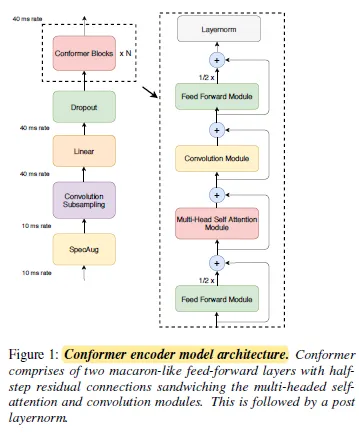
\includegraphics[width=\textwidth,height=0.7\textheight,keepaspectratio]{images/audio-nlp/transformer_conformer_overview.png}
                \caption*{\scriptsize Source: Gulati et al., ``Conformer'', Interspeech 2020, Fig.~1.}
            \end{figure}
        \end{column}
    \end{columns}
\end{frame}

\begin{frame}{What Changes When the Input Is Audio}
    The encoder blocks are the ones covered earlier. Two things about speech force adjustments:
    \begin{itemize}
        \setlength{\itemsep}{0.8em}
        \item \textbf{The sequence is very long.} At a 10~ms hop, one second of audio is 100 frames and a 30-second utterance is 3000, against perhaps 60 word-pieces of transcript. Self-attention costs $O(T^2)$, so ASR encoders first apply \textbf{convolutional subsampling}, typically two strided convolutions that cut the frame rate by $4\times$ (10~ms $\rightarrow$ 40~ms) before any attention layer runs.
        \item \textbf{Position matters relatively, not absolutely.} An utterance can start at any offset and last any length, so Conformer replaces absolute positional encoding with the \textbf{relative} sinusoidal scheme, making a block's behaviour depend on the distance between frames rather than their index.
    \end{itemize}
    \vspace{0.4em}
    Data augmentation on the input is also standard: \textbf{SpecAugment} masks bands of frequency and spans of time directly in the log-mel spectrogram.
\end{frame}

\begin{frame}{Conformer Block (Gulati et al., 2020)}
    \begin{itemize}
        \item \textbf{Conformer} combines self-attention and convolution for effective speech modeling.
        \item \textbf{Block Structure:} two \emph{half-step} feed-forward modules sandwich the attention and convolution pair (the ``macaron'' arrangement):
        \begin{itemize}
            \item $\tfrac{1}{2}$Feed-Forward $\rightarrow$ Multi-Head Self-Attention $\rightarrow$ Convolution $\rightarrow$ $\tfrac{1}{2}$Feed-Forward $\rightarrow$ LayerNorm
        \end{itemize}
        \item \textbf{Key Features:}
        \begin{itemize}
            \item \textbf{Convolution Module:} LayerNorm $\rightarrow$ pointwise conv (expansion 2) $\rightarrow$ GLU $\rightarrow$ 1-D depthwise conv $\rightarrow$ BatchNorm $\rightarrow$ Swish $\rightarrow$ pointwise conv $\rightarrow$ dropout.
            \item Every sub-module is a pre-norm residual unit; attention uses relative sinusoidal positional encoding.
        \end{itemize}
    \end{itemize}
\end{frame}
